\documentclass[a4paper,12pt]{report}
\usepackage{listings}
\usepackage{graphicx}
\usepackage{color}
 
\definecolor{codegreen}{rgb}{0,0.6,0}
\definecolor{codegray}{rgb}{0.5,0.5,0.5}
\definecolor{codepurple}{rgb}{0.58,0,0.82}
\definecolor{backcolour}{rgb}{0.95,0.95,0.92}
 
\lstdefinestyle{mystyle}{
    backgroundcolor=\color{backcolour},   
    commentstyle=\color{codegreen},
    keywordstyle=\color{magenta},
    numberstyle=\tiny\color{codegray},
    stringstyle=\color{codepurple},
    basicstyle=\footnotesize,
    breakatwhitespace=false,         
    breaklines=true,                 
    captionpos=b,                    
    keepspaces=true,                 
    numbers=left,                    
    numbersep=5pt,                  
    showspaces=false,                
    showstringspaces=false,
    showtabs=false,                  
    tabsize=2,
    language=python
}
\lstset{style=mystyle}
\title{Tugas Chapter 4}
\author{Rayhan Yuda Lesmana}
\date{6 November 2019}


\begin{document}
\maketitle


\section{Teori}
\section*{Pengenalan CSV}
\paragraph*{}
file csv Format file csv Comma Separated Values yaitu suatu
format data pada basis data dimana setiap record yang dapat dipisahkan dengan
menggunakan tanda koma (‘,) atau juga bisa dengan menggunakan titik
koma (‘;) sebagai tanda pemisah antara datu elemen dengan elemen yang
lainnya. Selain bahasa programnya yang sederhana, format ini juga dapat
dibuka dengan menggunakan berbagai text-editor seperti Notepad, Wordpad,
dan MS Excel.\\
Contoh file CSV:\\
\begin{figure}[h]
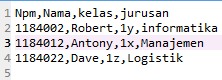
\includegraphics[scale=0.8]{gambar/1.png}
\end{figure}

\section*{Aplikasi yang dapat membuat file CSV}
\paragraph{}
\begin{enumerate}
\item Text editor (Notepat, Wordpad, dan lain-lain)
\item Spreadsheet (Microsoft Excel)
\end{enumerate}

\section*{Membuat dan membaca file csv di excel}


\begin{enumerate}
\item Membuka microsoft dan membuat dokumen baru.
\newpage
\item Tambahkan judul kolom untuk setiap potongan informasi yang ingin ditampilkan,
contohnya npm, nama, kelas, jurusan. Lalu ketikkan informasi keadalam kolom sesuai dengan judul nya.\\

\begin{figure}[h]
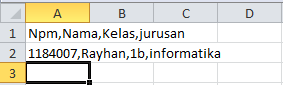
\includegraphics[scale=0.8]{gambar/2.png}
\end{figure}

\item Save file nya.
\begin{figure}[h]
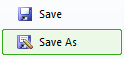
\includegraphics[scale=0.8]{gambar/3.png}
\end{figure}

\item Berinama file nya dan pilih extensi nya csv.
\begin{figure}[h]
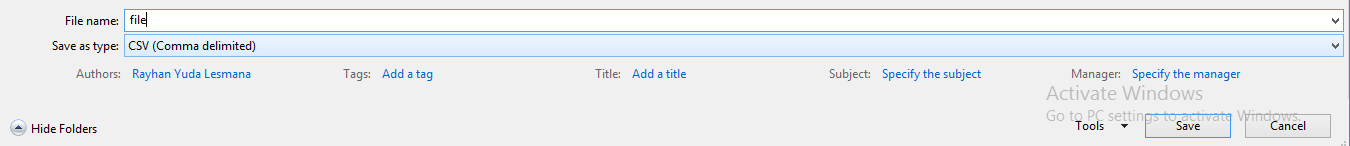
\includegraphics[scale=0.3]{gambar/4.png}
\end{figure}
\newpage
\item pilih yes.
\begin{figure}[h]
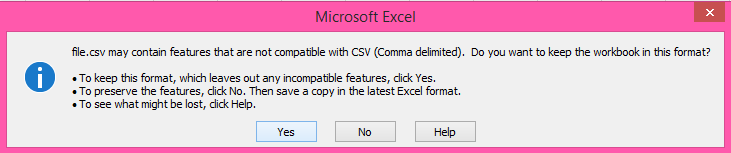
\includegraphics[scale=0.3]{gambar/5.png}
\end{figure}

\item file telah terbuat.
\begin{figure}[h]

\includegraphics[scale=0.8]{gambar/6.png}
\end{figure}
\end{enumerate}

\newpage
\begin{enumerate}
\item click pada file csv.
\begin{figure}[h]

\includegraphics[scale=0.8]{gambar/e.png}
\end{figure}
\item file telah terbuka.
\begin{figure}[h]
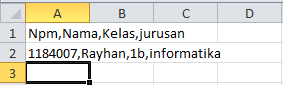
\includegraphics[scale=0.8]{gambar/r.png}
\end{figure}
\end{enumerate}

\section*{sejarah library csv}
\paragraph{}
Format yang disebut CSV Comma Separated Values
adalah format impor dan ekspor paling umum untuk spreadsheet dan basis
data. Format CSV digunakan selama bertahun-tahun sebelum upaya untuk
menggambarkan format dengan cara standar di RFC 4180. Kurangnya standar
yang didefinisikan dengan baik berarti bahwa perbedaan halus sering ada dalam
data yang diproduksi dan dikonsumsi oleh aplikasi yang berbeda.
Hal ini memungkinkan programmer untuk mengatakan, ”tulis data ini dalam
format yang disukai oleh Excel,” atau ”baca data dari file ini yang dihasilkan
oleh Excel ,” without knowing the correct details of the CSV format used
by Excel. Pemrogram juga dapat menggambarkan format CSV yang
RAHMATUL RIDHA 5
dipahami oleh aplikasi lain atau menentukan format CSV tujuan khusus mereka
sendiri.

\section*{sejarah library pandas}
\paragraph*{}
Pandas adalah alat sebagai analisis data dan struktur untuk bahasa pemrograman Python. Dengan menggunakan pandas kita dapat mengolah data dengan mudah, salah satu fiturnya adalah Dataframe. Dengan adanya fitur dataframe kita dapat membaca sebuah file dan menjadikannya table, kita juga dapat mengolah suatu data Banyak format file yang dapat dibaca menggunakan Pandas, seperti file .txt, .csv, .tsv dan lainnya. Agar lebih jelas mari
kita mencobanya secara langsung.

\section*{fungsi-fungsi yang terdapat di library csv}
\begin{enumerate}

\item reader: untuk membaca isi file berformat CSV dari list.
\begin{figure}[h]
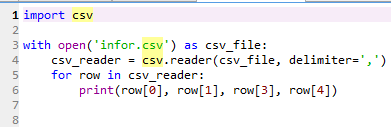
\includegraphics[scale=0.5]{gambar/7.png}
\end{figure}

\item DictReader:untuk membaca isi file berformat CSV dari dictionary.
\begin{figure}[h]
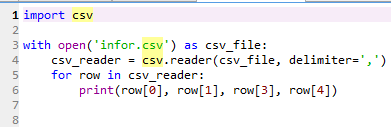
\includegraphics[scale=0.5]{gambar/7.png}
\end{figure}

\item write: untuk menulis file berformat CSV dari list.
\begin{figure}[h]

\includegraphics[scale=0.5]{gambar/8.png}
\end{figure}
\newpage
\item DictWrite:untuk menulis file berformat CSV dari dictionary.
\begin{figure}[h]

\includegraphics[scale=0.5]{gambar/8.png}
\end{figure}
\end{enumerate}

\section*{fungsi-fungsi yang terdapat di library pandas}
\begin{enumerate}

\item read csv:untuk membaca isi file berformat CSV
\begin{figure}[h]
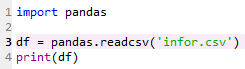
\includegraphics[scale=0.5]{gambar/9.png}
\end{figure}

\item to csv:untuk menulis file berformat CSV.
\begin{figure}[h]
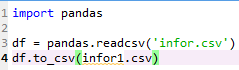
\includegraphics[scale=0.5]{gambar/10.png}
\end{figure}
\end{enumerate}

\section*{Keterampilan Pemograman}
\subsection*{Soal 1}
\paragraph{}Buatlah fungsi (le terpisah/library dengan nama NPM csv.py) untuk membuka le csv dengan lib csv mode list.
\lstinputlisting[language=Python, firstline=3, lastline=8]{src/1184007csv.py}

\subsection*{Soal 2}
\paragraph{}Buatlah fungsi (le terpisah/library dengan nama NPM csv.py) untuk membuka le csv dengan lib csv mode dictionary.
\lstinputlisting[language=Python, firstline=10, lastline=24]{src/1184007csv.py}

\subsection*{Soal 3}
\paragraph{}Buatlah fungsi (le terpisah/library dengan nama NPM pandas.py) untuk membuka le csv dengan lib pandas mode list
\lstinputlisting[language=Python, firstline=3, lastline=6]{src/1184007pandas.py}

\subsection*{Soal 4}
\paragraph{}Buatlah fungsi (le terpisah/library dengan nama NPM pandas.py) untuk membuka le csv dengan lib pandas mode dictionary.
\lstinputlisting[language=Python, firstline=8, lastline=12]{src/1184007pandas.py}

\subsection*{Soal 5}
\paragraph{}Buat fungsi baru di NPM pandas.py untuk mengubah format tanggal menjadi standar dataframe.
\lstinputlisting[language=Python, firstline=14, lastline=17]{src/1184007pandas.py}

\subsection*{Soal 6}
\paragraph{}Buat fungsi baru di NPM pandas.py untuk mengubah index kolom.
\lstinputlisting[language=Python, firstline=19, lastline=23]{src/1184007pandas.py} 

\subsection*{Soal 7}
\paragraph{}Buat fungsi baru di NPM pandas.py untuk mengubah atribut atau nama kolom.
\lstinputlisting[language=Python, firstline=25, lastline=37]{src/1184007pandas.py}   

\subsection*{Soal 8}
\paragraph{}Buat program main.py yang menggunakan library NPM csv.py yang membuat dan membaca file csv.
\lstinputlisting[language=Python, firstline=1, lastline=7]{src/main.py}

\subsection*{Soal 9}
\paragraph{}Buat program main2.py yang menggunakan library NPM pandas.py yang membuat dan membaca file csv.
\lstinputlisting[language=Python, firstline=9, lastline=15]{src/main.py}
        
\section*{Plagiarism}
\begin{figure}[h]
\begin{center}
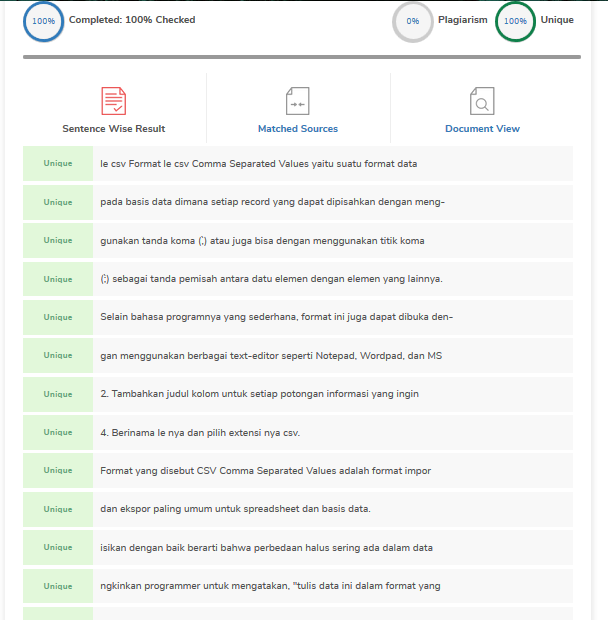
\includegraphics[scale=0.8]{gambar/11.png}
\end{center}
\end{figure}
 
        
        
        
        


\end{document}